\section{Case Study}
\label{sec:case}

%%\wrm{Re-do case studies in Bud} \wrm{Break cart development down into
%%iterations} \wrm{How does the language naturally lead us to an order
%%independent style?  Talk about inserting all sorts of exotic stuff like queues
%%if we want a highly order-dependent imperative style.}

\jmh{We discussed the following on the phone.  (1) Handle shopping in two styles: destructive updates, and disorderly accumulation of increment/decrement.  (2) Do analysis on them to detect need for coordination in only the first, show that (annotated) 2PC removes the compiler warning.  (3) Deploy destructive+2PC on EC2 and show practical benefits of avoiding coordination.  (4) Evolve the program with new rules for checkout and/or inventory, show how the disorderly version is no longer monotonic.  Fix that  with 2PC where needed.  Also make sure the destructive version works with the new rules.  Now show that the disorderly version is still better than the destructive one, by coordinating only where needed.}

\jmh{Finally, show what would happen if you didn't coordinate the inventory bit, but tracked taint.  Note that tainted output is the stuff where programmers need to write compensation logic.}


In this section, we implement two different styles of distributed shopping cart
applications in Bud.  First, we implement a ``destructive,'' overwriting
shopping cart application using a simple key-value store implemented in Bud.
Second, we implement a ``disorderly'' cart which accumulates updates in a 
set-wise fashion and describes how to combine the updates into a final result.

For each, we apply whole-program analysis techniques to discover points of 
order in the program.  The analysis, based on traditional stratification
techniques, represents the dependency graph of predicates (and hence the 
flow of tuples) as a staged dataflow graph.  Asynchronous message sending
is indicated by a dotted line in the graph, while edges that involve 
nonmonotonic logic are marked with a $\lnot$.  Edges that involve a temporal 
edge are marked with a $+$.  Strongly connected components having both a $\lnot$ and a $+$ edge are grouped into temporal clusters.  Individual monotonic components 
(or strata) are surrounded by a dashed rectangle.  A point of order occurs
whereever an edge crosses strata, or at any self-edge attached to a temporal cluster.



\subsection{Destructive Cart}

\begin{figure}[t]
\centering
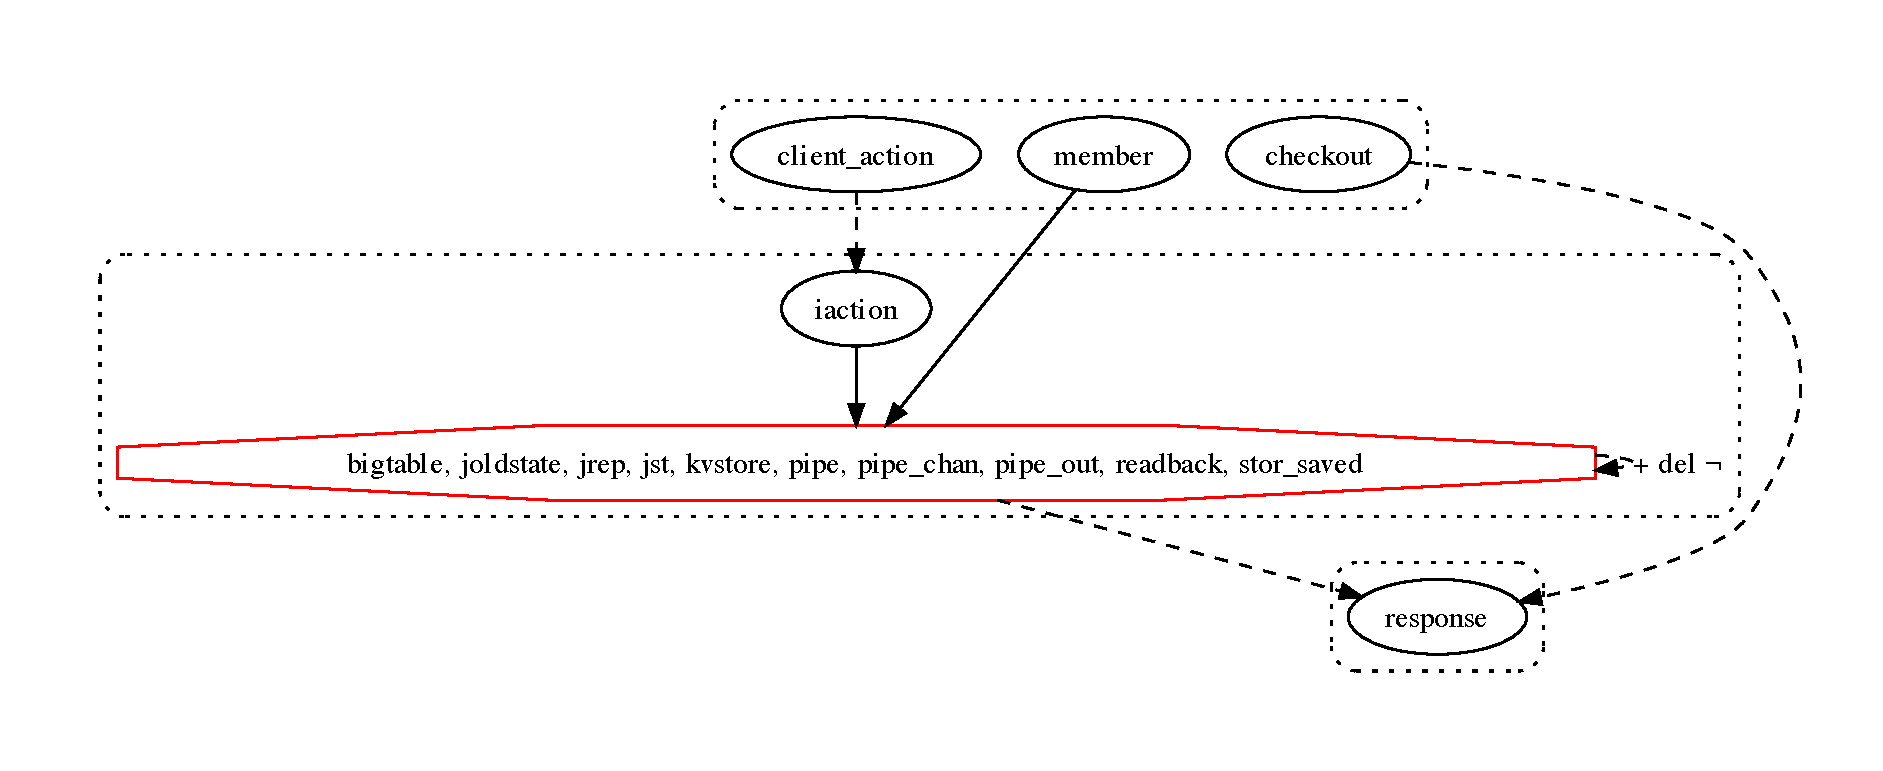
\includegraphics[width=1.2\linewidth]{fig/ImperativeCartServer_gvoutput.pdf}
\caption{Destructive Cart (cycles collapsed)}
\label{fig:cs-pgd-1}
\end{figure}

Note the points of order between \emph{client\_action} and \emph{iaction}
and between the temporal cluster and itself.



\subsection{Disorderly Cart}

\begin{figure}[t]
\centering
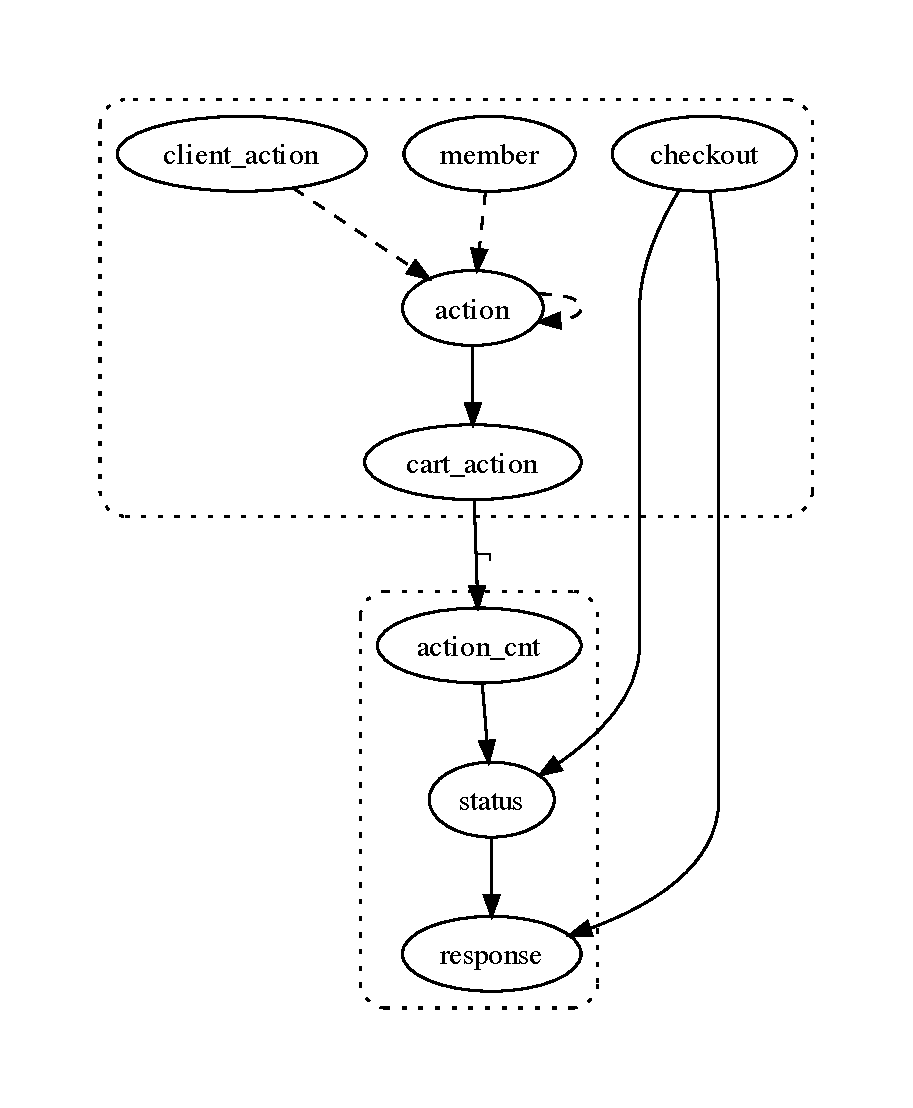
\includegraphics[width=0.9\linewidth]{fig/BasicCartServer_gvoutput.pdf}
\caption{Disorderly Cart}
\label{fig:cs-pgd-1}
\end{figure}




